\chapter{Evaluation}
\label{ch:evaluation}
The hclm cluster was used to evaluate the performance of DIIS for mixing the self-energy. We decided to use reasonable small calculations that would finish in a few hours.

The chosen hamilton was given by a hubbard square with $80\times80$ sites, half filling, $U=8$ and $\beta=50$.

\lstdefinelanguage{ini}{
  basicstyle=\ttfamily\small,
  columns=fullflexible,
  morecomment=[s][\color{Orchid}\bfseries]{[}{]},
  morecomment=[s][\color{Orchid}\bfseries]{[[}{]]},
  morecomment=[l]{\#},
  morecomment=[l]{;},
  commentstyle=\color{gray}\ttfamily,
  morekeywords={},
  keywordstyle={\color{green}\bfseries}
}

\begin{lstlisting}[label=lst:w2dyn_config, language=ini, caption=The w2dynmaics configuration for this case]
[General]
DOS=ReadIn
HkFile=hubbard_2d_80_80_1.hk
beta=50.
NAt=1
totdens=1.
EPSN=0
mu=4.0
DMFTsteps=50
StatisticSteps=0
FileNamePrefix=square_u08_b50_diis
magnetism=para
siw_moments=estimate
FTType=none
mixing=0.0
mixing_strategy=diis
mixing_diis_history=5
mixing_diis_period=1

[Atoms]
[[1]]
Hamiltonian=Density
Udd=8.0
Nd=1

[QMC]
Nwarmups=1e6
Nmeas=1e5
NCorr=200
Ntau=1000
Niw=2000
Eigenbasis=1 
MeasGiw=1
\end{lstlisting}

The baseline was given by the same configuration, but without DIIS mixing.

\begin{figure}[H]
    \centering
    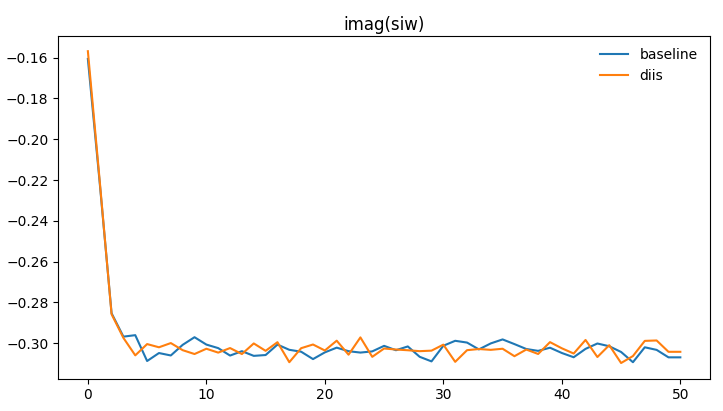
\includegraphics[width=1.0\textwidth]{figures/square_u08_b50_siw_imag.png}
    \caption{DMFT iteration comparison for matsubara frequency 0}
    \label{fig:dmft}
\end{figure}

